\documentclass{article}
\usepackage[backend=biber,citestyle=ieee]{biblatex}
\usepackage[english]{babel}
% \usepackage[swedish]{babel}
\usepackage{graphicx}
\usepackage{csquotes}
\usepackage{float}
\usepackage{datetime}
\usepackage[title]{appendix}
% \usepackage{a4wide} %For wider content on page
% \usepackage{amsmath} %For multiline equations 

\usepackage{fancyhdr}   %page header
\pagestyle{fancy}

% \usepackage[parfill]{parskip} %Line skip between paragraphs instead of indent

\usepackage{xcolor}
\usepackage{listings}

\definecolor{codegreen}{rgb}{0,0.6,0}
\definecolor{codegray}{rgb}{0.5,0.5,0.5}
\definecolor{codepurple}{rgb}{0.58,0,0.82}
\definecolor{backcolour}{rgb}{0.95,0.95,0.95}
\lstdefinestyle{mystyle}{
    backgroundcolor=\color{backcolour},   
    commentstyle=\color{codegreen},
    keywordstyle=\color{magenta},
    numberstyle=\tiny\color{codegray},
    stringstyle=\color{codepurple},
    basicstyle=\ttfamily\footnotesize,
    breakatwhitespace=false,         
    breaklines=true,                 
    captionpos=b,                    
    keepspaces=false,                 
    numbers=left,                    
    numbersep=5pt,                  
    showspaces=false,                
    showstringspaces=false,
    showtabs=false,                  
    tabsize=1
}
\lstset{style=mystyle}

%\addbibresource{sources.bib}

\newcommand{\getauthor}{Elias Berglin} %Author
\newcommand{\gettitle}{Lab 2: MQTT} %Title

\newdateformat{daymonthyear}{\ordinal{DAY} \monthname[\THEMONTH] \THEYEAR} %Date

\title{\gettitle}
\author{\getauthor}

\date{\daymonthyear\today} %Remove for swedish date

\begin{document}

    % Title 
    \pagenumbering{gobble}
    \maketitle
    \newpage

    % Page header and footer
    \pagenumbering{arabic}
    \fancyhf{}
    \lhead{\getauthor}
    \rhead{\gettitle}
    \rfoot \thepage

    % Document starts here
    \section{Pre-defined messages}
    As I am building the broker part of the MQTT system there will be a lot of fixed responses. The complete code can be found in appendix \ref{appendix:code}. The two most important responses will be connection ACK and ping ACK. We need these to connect and keep the connection alive. In figure \ref{fig:ackCode} we can see that all these functions do is create a byte array containing the bytes needed to respond.
    \begin{figure}[H]
        \label{fig:ackCode}
    \begin{lstlisting}[language=go]
func createConnectionAccept() []byte {
	var message []byte
	message = append(message, byte(0b00100000))
	message = append(message, byte(0b00000010))
	message = append(message, byte(0x0))
	message = append(message, byte(0x0))
	return message
}
func createPingAck() []byte {
	var message []byte
	message = append(message, byte(0b11010000))
	message = append(message, byte(0x0))
	return message
}
    \end{lstlisting}
    \caption{Go code for create ACK for connect and ping}
\end{figure}

\newpage
\section{Parsing incoming message}
In figure \ref{fig:parseCode} is the code for parsing a subscribe message. It is important to keep in mind that a subscribe message can contain multiple topics and thus this needs to be checked. The function returns three values. First it returns if the subscription was successful, so we can pass that data to the ACK. The second return parameter is the identifier for the message that is later passed to subscribe ACK. The last return is a list of all the topics that the client subscribed to. The way that I parse the message here is I pop the number of bytes I want from the array. Go does not provide a simple way to do this. If we look at row 9 in figure \ref{fig:parseCode} we can see that I have an assignment of two variables. The variable l in this case is the bytes representing the length of the topic and body is the message body and is overwritten. On the right side of the equals sign I first assign the two bytes to l and then assign the remaining bytes to body, and thus I have popped the front of the array.
\begin{figure}[H]
    \begin{lstlisting}[language=go]
func parseSubscribe(message []byte, c *net.Conn, id string) (bool, []byte, []string) {
	body := message[2:]
	var l []byte
	var subscribe string
	var qos int
	var subs []string

	for len(body) > 0 {
		l, body = body[:2], body[2:]
		subLen := binary.BigEndian.Uint16(l)
		if len(body) < int(subLen) {
			return false, message[:2], nil
		}
		subscribe, body = string(body[:subLen]), body[subLen:]
		if len(body) == 0 {
			return false, message[:2], nil
		}
		addSubscription(c, subscribe)
		subs = append(subs, subscribe)
		qos, body = int((body[0] & 0b00000011)), body[1:]
		fmt.Println(DEVIDER)
		fmt.Println(id+" subscribed to: "+subscribe+" \nWith QOS of:", qos)
		fmt.Println(DEVIDER)
		fmt.Println()
	}
	return true, message[:2], subs
}
    \end{lstlisting}
    \label{fig:parseCode}
    \caption{Go code for parsing a subscribe message}
\end{figure}

\newpage
\section{Broadcaster}
To make sure all the connections get the messages they subscribed to I implemented a broadcaster. This function is responsible for delivering published data to all the subscribed clients. To help with this I have a global map with string keys and an array of pointers to connection as value. To know when to send data the broadcaster listens to a channel. A channel in go is a way for threads to communicate with one another. When a publish is received the packet along with information is sent on the channel and is picked up by the broadcaster. When the broadcaster receives the message it can get the list of pointers from the global map and iterate through them and send the packet to each subscriber. The broadcaster code can be found in figure \ref{fig:broadFunc}. 
\begin{figure}[H]
    \begin{lstlisting}[language=go]
func broadcaster(ch chan BroadCastMessage) {
	for {
		message := <-ch
		connections := subscriptions[message.Topic]
		if len(connections) <= 0 {
			continue
		}
		fmt.Println(DEVIDER)
		fmt.Println("Broadcasting message to: ",
			message.Topic, "\ncontaining ", message.Message)
		fmt.Println(DEVIDER)
		fmt.Println()
		for _, c := range subscriptions[message.Topic] {
			(*c).Write(message.Packet)
		}
	}
}
    \end{lstlisting}
    \label{fig:broadFunc}
    \caption{Go code for the broadcaster function}
\end{figure}

\newpage
\section{Main function}
The main function is responsible to set up the broadcast function, initiate the global video and accept incoming connections. The code can be found in figure \ref{fig:mainGO}. In row 8 I initialize the channel that is used by the broadcaster and on line 9 I use the go keyword to run the broadcaster function in a new thread. I use the same keyword on line 22 where I hand over the connection to a new thread and then the function goes back to handle new connections.
\begin{figure}[H]
    \begin{lstlisting}[language=go]
func main() {
	deviderLen := 50
	for i := 0; i < deviderLen; i++ {
		DEVIDER += "-"
	}
	subscriptions = make(map[string][]*net.Conn)
	lastValue = make(map[string][]byte)
	ch := make(chan BroadCastMessage)
	go broadcaster(ch)
	port := ":1883"
	s, err := net.Listen("tcp", port)
	if err != nil {
		panic(err)
	}
	defer s.Close()

	for {
		c, err := s.Accept()
		if err != nil {
			panic(err)
		}
		go acceptMessage(&c, ch)
	}
}
    \end{lstlisting}
    \caption{The main go function}
    \label{fig:mainGO}
\end{figure}

\newpage
\section{Flowchart}
Figure \ref{fig:MQTT} represents the flowchart for the program.
\begin{figure}[H]
	\centering
    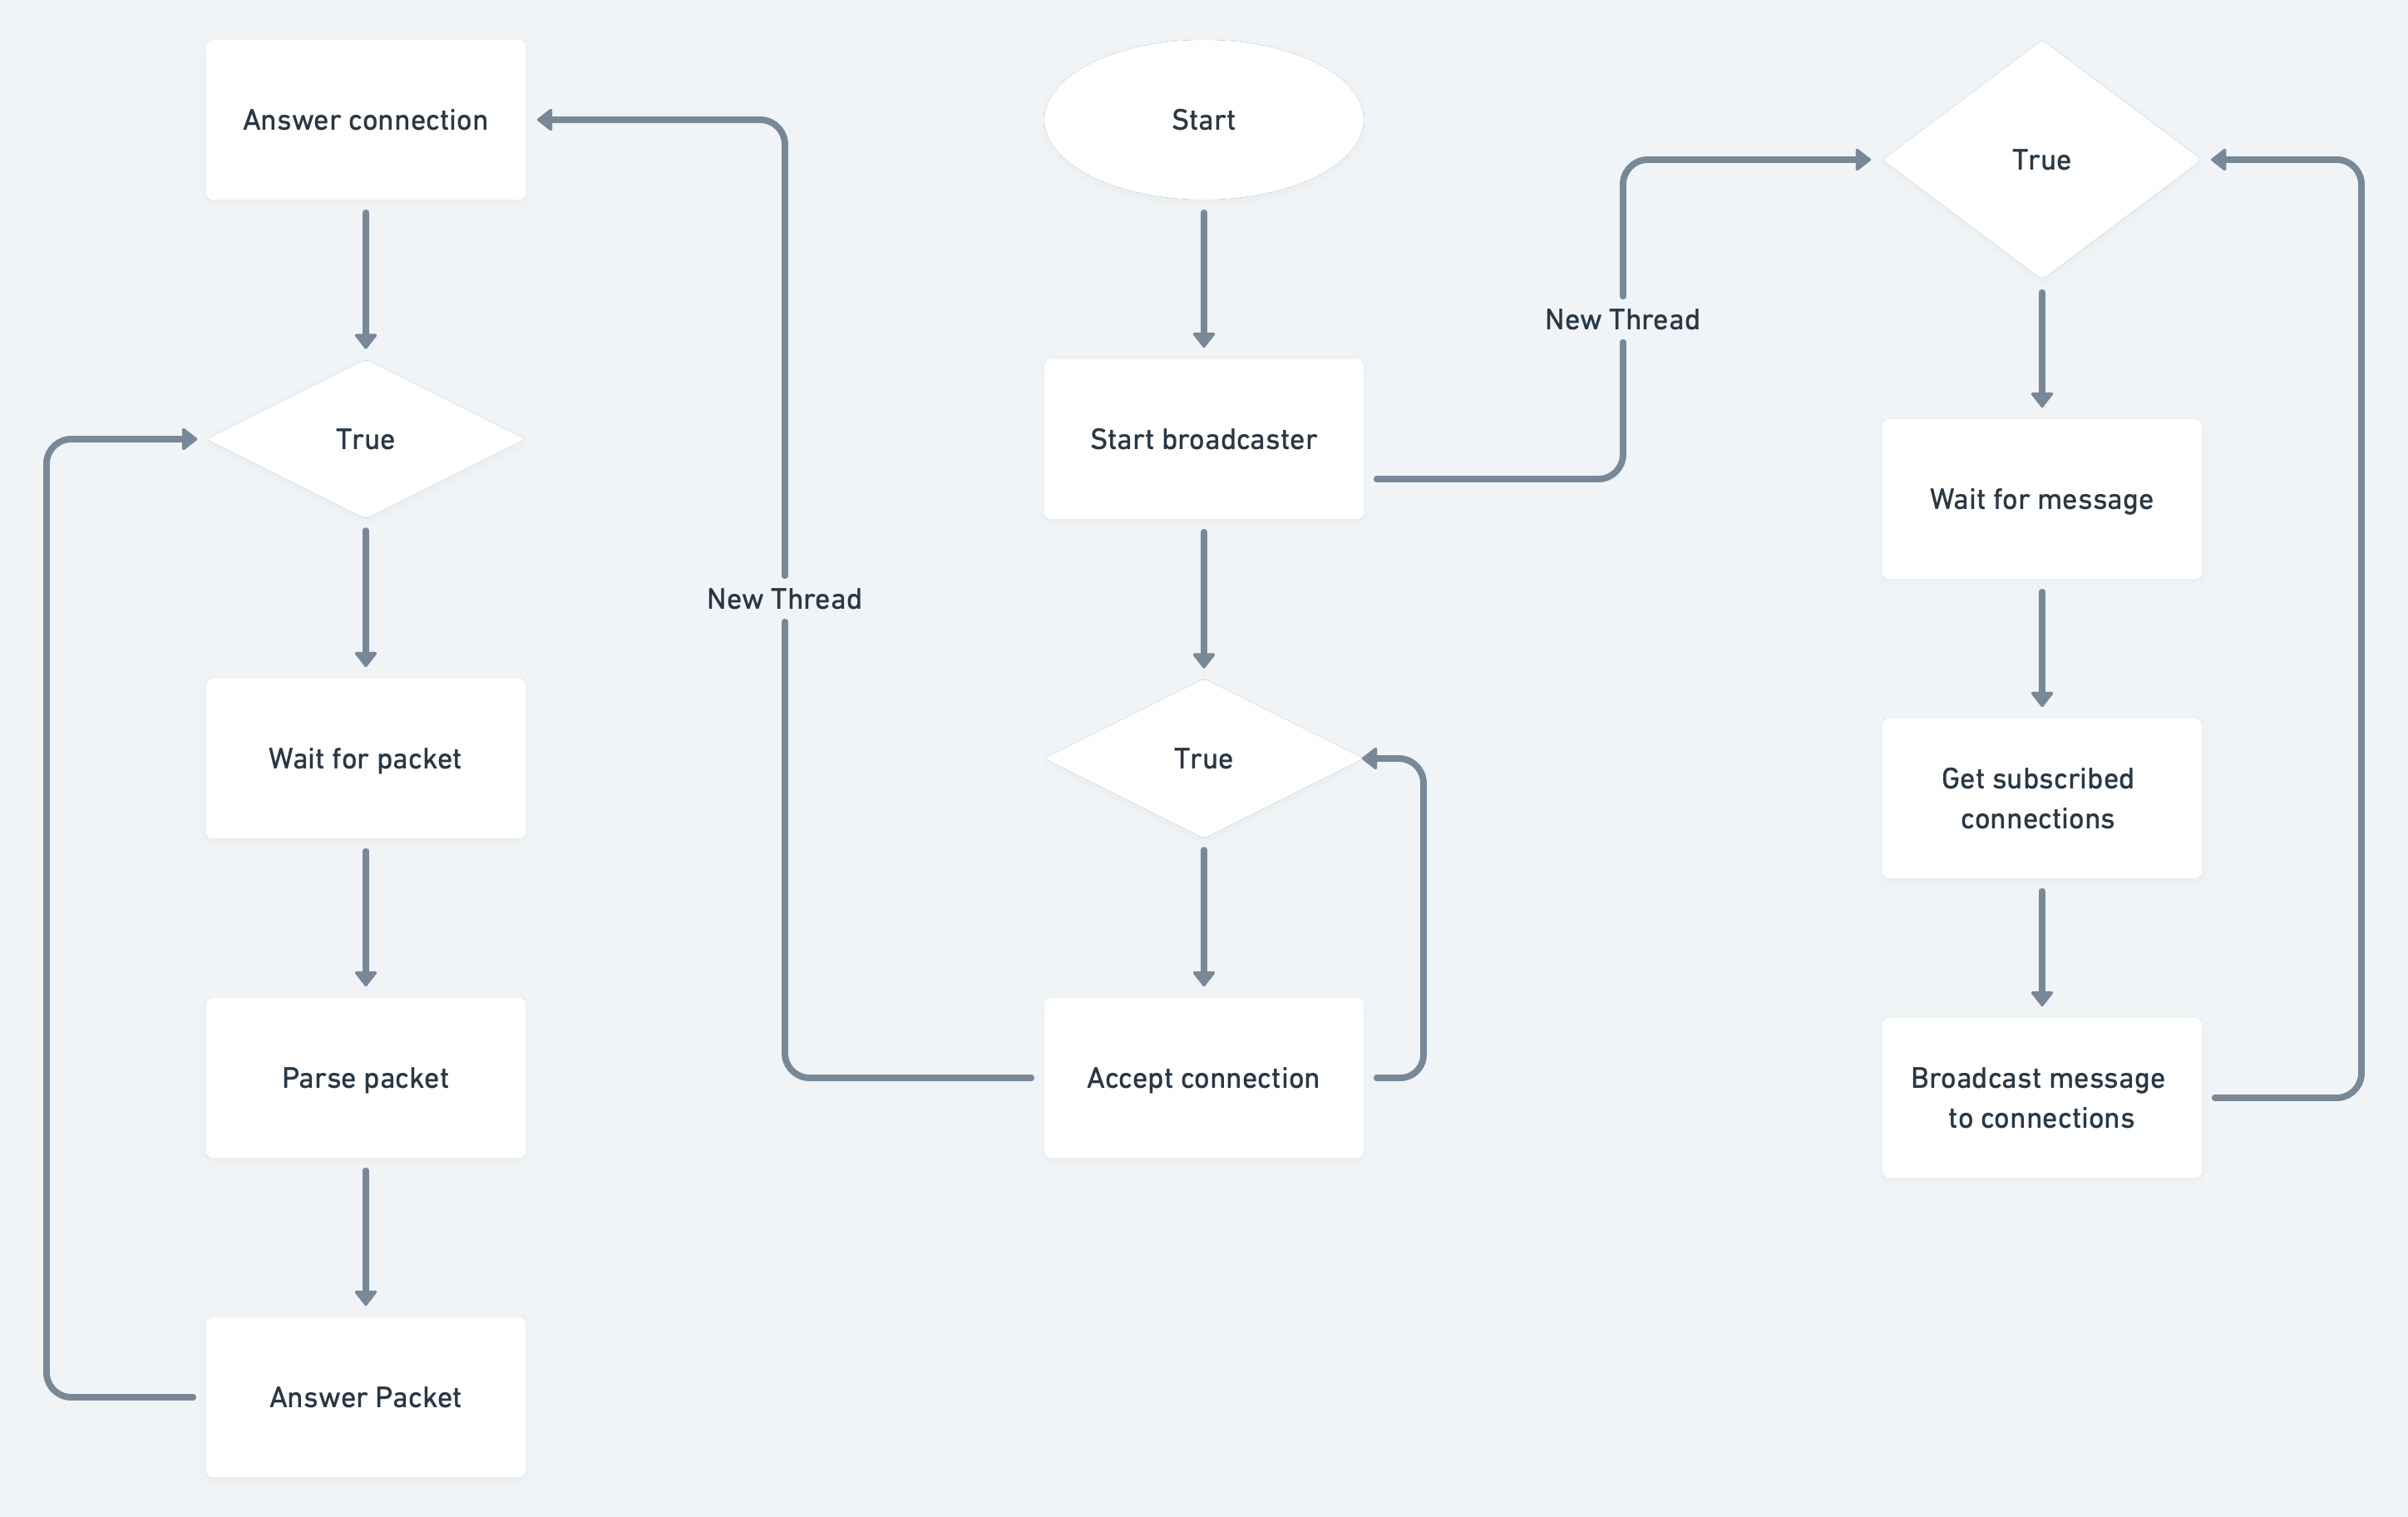
\includegraphics[width=1\textwidth]{MQTT2.png}
	\label{fig:MQTT}
	\caption{Flow of the MQTT broker}
\end{figure}

    % Appendices
    \newpage
    \begin{appendices}

        \section{Code}
        \label{appendix:code}
        \begin{lstlisting}[language=go]
package main

import (
	"encoding/binary"
	"fmt"
	"net"
	"strconv"
)

var subscriptions map[string][]*net.Conn
var lastValue map[string][]byte
var DEVIDER string

type BroadCastMessage struct {
	Topic   string
	Message string
	Packet  []byte
}

func broadcaster(ch chan BroadCastMessage) {
	for {
		message := <-ch
		connections := subscriptions[message.Topic]
		if len(connections) <= 0 {
			continue
		}
		fmt.Println(DEVIDER)
		fmt.Println("Broadcasting message to: ",
			message.Topic, "\ncontaining ", message.Message)
		fmt.Println(DEVIDER)
		fmt.Println()
		for _, c := range subscriptions[message.Topic] {
			(*c).Write(message.Packet)
		}
	}
}

func addSubscription(c *net.Conn, filter string) {
	if subscriptions[filter] == nil {
		subscriptions[filter] = make([]*net.Conn, 0)
	}
	subscriptions[filter] = append(subscriptions[filter], c)
}

func removeSubscription(c *net.Conn, filter string) {
	conns := subscriptions[filter]
	var newConns []*net.Conn

	for _, conn := range conns {
		if conn != c {
			newConns = append(newConns, conn)
		}
	}
	subscriptions[filter] = newConns
}

func removeAllSubs(c *net.Conn) {
	for topic, conns := range subscriptions {
		var newConns []*net.Conn
		for _, conn := range conns {
			if conn != c {
				newConns = append(newConns, conn)
			}
		}
		subscriptions[topic] = newConns
	}
}

func createConnectionAccept() []byte {
	var message []byte
	message = append(message, byte(0b00100000))
	message = append(message, byte(0b00000010))
	message = append(message, byte(0x0))
	message = append(message, byte(0x0))
	return message
}
func createPingAck() []byte {
	var message []byte
	message = append(message, byte(0b11010000))
	message = append(message, byte(0x0))
	return message
}

func createSubAck(identifier []byte, success bool) []byte {
	var message []byte
	message = append(message, byte(0b10010000))
	message = append(message, byte(0b00000011))
	message = append(message, identifier...)
	if success {
		message = append(message, byte(0x00))
	} else {
		message = append(message, byte(0x80))
	}

	return message
}

func createUnsubAck(identifier []byte) []byte {
	var message []byte
	message = append(message, byte(0b10110000))
	message = append(message, byte(0x2))
	message = append(message, identifier...)
	return message
}

func parseSubscribe(message []byte, c *net.Conn, id string) (bool, []byte, []string) {
	body := message[2:]
	var l []byte
	var subscribe string
	var qos int
	var subs []string

	for len(body) > 0 {
		l, body = body[:2], body[2:]
		subLen := binary.BigEndian.Uint16(l)
		if len(body) < int(subLen) {
			return false, message[:2], nil
		}
		subscribe, body = string(body[:subLen]), body[subLen:]
		if len(body) == 0 {
			return false, message[:2], nil
		}
		addSubscription(c, subscribe)
		subs = append(subs, subscribe)
		qos, body = int((body[0] & 0b00000011)), body[1:]
		fmt.Println(DEVIDER)
		fmt.Println(id+" subscribed to: "+subscribe+" \nWith QOS of:", qos)
		fmt.Println(DEVIDER)
		fmt.Println()
	}
	return true, message[:2], subs
}

func parseUnsubscribe(message []byte, c *net.Conn, id string) []byte {
	body := message[2:]
	var l []byte
	var unSub string
	for len(body) > 0 {
		l, body = body[:2], body[2:]
		subLen := binary.BigEndian.Uint16(l)
		unSub, body = string(body[:subLen]), body[subLen:]
		removeSubscription(c, unSub)
		fmt.Println(DEVIDER)
		fmt.Println(id + " unsubscribed from: " + unSub)
		fmt.Println(DEVIDER)
		fmt.Println()
	}
	return message[:2]
}

func parsePublish(message []byte, retain bool, id string) (string, string) {
	data := ""
	topic := ""
	var topicLenBytes []byte

	topicLenBytes, message = message[:2], message[2:]
	topicLength := binary.BigEndian.Uint16(topicLenBytes)
	topic, message = string(message[:topicLength]), message[topicLength:]

	data = string(message)
	fmt.Println(DEVIDER)
	fmt.Println(id + " publshed: ")
	fmt.Println("Topic: ", topic)
	fmt.Println("Data: ", data)
	fmt.Println("Will retain: ", retain)
	fmt.Println(DEVIDER)
	fmt.Println()

	return data, topic
}

func handleConnection(c *net.Conn, ch chan BroadCastMessage, id string) {
	fmt.Println(DEVIDER)
	fmt.Println("Accepting connection from: " + id)
	fmt.Println(DEVIDER)
	fmt.Println()
	conAck := createConnectionAccept()
	(*c).Write(conAck)
	for {
		constHEAD := make([]byte, 2)
		(*c).Read(constHEAD)
		messageType := int((constHEAD[0] & 0b11110000) >> 4)
		switch messageType {
		case 12: //Ping
			fmt.Println(DEVIDER)
			fmt.Println("Answering Ping Request from: " + id)
			fmt.Println(DEVIDER)
			fmt.Println()
			pingAck := createPingAck()
			(*c).Write(pingAck)
			break
		case 14: // Disconect
			fmt.Println(DEVIDER)
			fmt.Println("Disconnecting: " + id)
			fmt.Println(DEVIDER)
			fmt.Println()
			removeAllSubs(c)
			(*c).Close()
			return
		case 8: // Subscribe
			remainder := int(constHEAD[1])
			messageArr := make([]byte, remainder)
			(*c).Read(messageArr)
			success, code, subs := parseSubscribe(messageArr, c, id)
			subAck := createSubAck(code, success)
			for _, s := range subs {
				if len(lastValue[s]) == 0 {
					continue
				}
				(*c).Write(lastValue[s])
			}
			(*c).Write(subAck)
			break
		case 10: // Unsubscribe
			remainder := int(constHEAD[1])
			messageArr := make([]byte, remainder)
			(*c).Read(messageArr)
			(*c).Write(createUnsubAck(parseUnsubscribe(messageArr, c, id)))
			break
		case 3: // Publish
			remainder := int(constHEAD[1])
			messageArr := make([]byte, remainder)
			retain := int(constHEAD[0] & 0b00000001)
			qos := int((constHEAD[0] & 0b00000110) >> 1)
			if qos != 0 {
				fmt.Println("Unsuported QoS type")
				removeAllSubs(c)
				(*c).Close()
				return
			}
			(*c).Read(messageArr)
			data, topic := parsePublish(messageArr, retain != 0, id)
			ch <- BroadCastMessage{
				Message: data,
				Topic:   topic,
				Packet:  append(constHEAD, messageArr...),
			}
			if retain != 0 {
				lastValue[topic] = append(lastValue[topic],
					append(constHEAD, messageArr...)...)
			}
			break
		default:
			fmt.Println(DEVIDER)
			fmt.Println("Got message type: " + strconv.Itoa(messageType))
			fmt.Println("This is not handled by brooker")
			if messageType == 0 {
				fmt.Println("Message type 0 could be a forced disconect")
			}
			fmt.Println(DEVIDER)
			fmt.Println()
			removeAllSubs(c)
			(*c).Close()
			return
		}
	}
}

func acceptMessage(c *net.Conn, ch chan BroadCastMessage) {
	constHEAD := make([]byte, 2)
	(*c).Read(constHEAD)
	packetType := int((constHEAD[0] & 0b11110000) >> 4)
	remainder := int(constHEAD[1])
	if packetType != 1 {
		panic("Not a connection")
	}
	message := make([]byte, remainder)
	(*c).Read(message)
	mqttStringLen := binary.BigEndian.Uint16(message[:2])
	if mqttStringLen != 4 {
		(*c).Close()
		panic("Wrong protocoll")
	}
	mqttString := string(message[2:6])
	if mqttString != "MQTT" {
		(*c).Close()
		panic("Wring protocoll")
	}

	version := message[6]
	if version != 4 {
		panic("Protocoll not supported")
	}
	var payload []byte
	if len(message) > 10 {
		payload = message[10:]
	}
	id := "Null Identifier"
	if len(payload) > 0 {
		id = string(payload)
	}
	handleConnection(c, ch, id)
}

func main() {
	deviderLen := 50
	for i := 0; i < deviderLen; i++ {
		DEVIDER += "-"
	}
	subscriptions = make(map[string][]*net.Conn)
	lastValue = make(map[string][]byte)
	ch := make(chan BroadCastMessage)
	go broadcaster(ch)
	port := ":1883"
	s, err := net.Listen("tcp", port)
	if err != nil {
		panic(err)
	}
	defer s.Close()

	for {
		c, err := s.Accept()
		if err != nil {
			panic(err)
		}
		go acceptMessage(&c, ch)
	}
}

        \end{lstlisting}

    \end{appendices}

\end{document}

% list with a,b,c
% \begin{enumerate}[label=(\alph*)]
%     \item 
% \end{enumerate}

% Centered figure with caption:
% \begin{figure}[H]
%     \centering
%     \includegraphics[width=1\textwidth]{%path} 
%     \caption{}
%     \label{fig:}
% \end{figure}

% Side by side figures:
% \begin{figure}[H]
%     \centering
%     \subfloat{{\includegraphics[width=0.46\textwidth]{%path} }}%
%     \qquad
%     \subfloat{{\includegraphics[width=0.46\textwidth]{%path} }}%
%     \caption{}
%     \label{fig:}
% \end{figure}

% Table with caption:
% \begin{table}[H]      
%     \begin{center}
%     \begin{tabular}{|c|c|} 
%         \hline
%         \textbf{} & \textbf{} \\\hline\hline
%          &  \\\hline 
%     \end{tabular}
%     \end{center}
%     \caption{}
%     \label{tab:}
% \end{table}

% Equation on multiple lines
% \begin{equation}
%    \begin{split}
%        x &= y \\
%        y &= z
%    \end{split}
% \end{equation}

% Code snippet
% \begin{lstlisting}%[language=]
%    //Code here
% \end{lstlisting}

% Code snippet from source file 
% \lstinputlisting[language=]{%path}
